% Code:
%   src/sudoku_solver/solvers/backtracking/
%     naive.py       (solve, stack_solve, solve_steps)
%     heuristic.py   (MRV, Forward Checking)
%     counting.py    (Lösungsanzahl, Eindeutigkeit, Baumgröße)
%     estimation.py  (Knuth-Schätzer)
%   Zahlen für die Tabellen:
%   python -m sudoku_solver.solvers.backtracking.report


\section{Backtracking-Solver}\label{sec:bt}

Als erster der beiden Lösungsansätze wird in diesem Kapitel der Backtracker behandelt.
Hierfür wird das Sudoku als Entscheidungsproblem betrachtet, jedoch ist Backtracking ein
Suchverfahren, welches Schritt für Schritt eine konkrete Lösung konstruiert. 
Dafür wird das Sudoku als ein Suchproblem betrachtet, dessen Teillösungen einen Suchbaum bilden.

Als erstes werden die Grundlagen für das Entscheidungsproblem gelegt (Abschnitt \ref{sec:bt-suchbaum}),
anschließend wird der Algorithmus und seine Implementierung beschrieben (Abschnitt \ref{sec:bt-algorithmus}).
Daraufhin wird begründet, dass das Verfahren korrekt, vollständig und stets terminiert ist (Abschnitt \ref{sec:bt-korrektheit}),
und sein Bedarf an Laufzeit und Speicher eingeordnet (Abschnitt \ref{sec:bt-komplexitaet}).
Die letzten beiden Abschnitte behandeln Heuristiken um den Suchbaum zu verkleinern (Abschnitt \ref{sec:bt-heuristiken}),
sowie abschließend ein Verfahren nach Knuth, das die Größe des Suchbaums vor dem durchsuchen schätzt (Abschnitt \ref{sec:bt-knuth}). 

% ----------------------------------------------------------------------------
\subsection{Zustandsraum und Suchbaum}\label{sec:bt-suchbaum}

Grundlage des Backtrackings ist ein Zustandsraum, der die schrittweise entstehenden Teillösungen eines Sudokus beschreibt.
Dazu werden die $k$ leeren Zellen zeilenweise von links oben nach rechts unten als $z_1, \dots, z_k$ nummeriert. 
Ein \emph{Zustand} ist eine partielle Belegung, die den ersten $i$ dieser Zellen mit $0 \leq i \leq k$ 
jeweils eine Ziffer aus $\{1, \dots, 9\}$ zuordnet. 
Er heißt \emph{konsistent}, wenn zusammen mit den Vorgaben keine Zeile, keine Spalte und kein Block eine Ziffer mehrfach enthält. 
Eine Lösung ist damit ein konsistenter Zustand, der alle $k$ leeren Zellen belegt.

Die konsistenten Zustände bilden einen \emph{Suchbaum}. 
Seine Wurzel ist das Sudoku mit seinen Vorgaben, 
und die Kinder eines Knotens der Tiefe $i$ sind alle konsistenten Zustände, die ihn um eine Ziffer für $z_{i+1}$ erweitern. 
Jeder Knoten außer der Wurzel entspricht somit genau einer gesetzten Ziffer. 
Der Verzweigungsgrad, also die Anzahl der zulässigen Ziffern der nächsten Zelle, beträgt höchstens neun, 
die Tiefe des Baums höchstens $k$. 
Ein Blatt ist entweder eine Lösung oder eine \emph{Sackgasse}, 
also ein konsistenter Zustand, für dessen nächste Zelle keine Ziffer mehr zulässig ist.

Wie in Abschnitt~\ref{sec:komplexitaet} beschrieben, 
ließe sich die Lösbarkeit auch durch Prüfen aller $9^k$ vollständigen Belegungen entscheiden. 
Bei $k = 60$ leeren Zellen wären das jedoch etwa $1{,}8 \cdot 10^{57}$ Belegungen, 
für die selbst eine Milliarde Prüfungen pro Sekunde mehr als $10^{40}$ Jahre bräuchten. 
Backtracking vermeidet diesen Aufwand, indem es die Konsistenz bereits nach jeder gesetzten Ziffer prüft \vgl{russell2021}. 
Grundlage ist eine Monotonie-Eigenschaft: Enthält ein Zustand einen Widerspruch, so enthält ihn auch jede seiner Erweiterungen. 
Ein inkonsistenter Zustand wird daher gar nicht erst erzeugt, 
und mit ihm entfällt sein gesamter Teilbaum mit bis zu $9^{k-i}$ Belegungen. 
Dieses Abschneiden wird als \emph{Pruning} bezeichnet.

Backtracking ist also eine Tiefensuche auf dem Suchbaum; 
Der aktuelle Zustand wird so lange um zulässige Ziffern erweitert, bis eine Lösung oder eine Sackgasse erreicht ist. 
In einer Sackgasse wird die zuletzt gesetzte Ziffer zurückgenommen und im Elternknoten die nächste Alternative probiert. 
Diesem Rücksprung verdankt das Verfahren seinen Namen ("Backtracking"). 
Der Suchbaum wird dabei nie vollständig gespeichert, sondern während der Suche schrittweise erzeugt. 
Abbildung~\ref{fig:bt-suchbaum} zeigt dies am vollständigen Suchbaum eines $4 \times 4$-Sudokus 
mit den Ziffern 1 bis 4 und $k = 5$ leeren Zellen: 
Statt der $4^5 = 1024$ möglichen Belegungen setzt das Backtracking nur sieben Ziffern 
und durchläuft zwei Sackgassen, bevor es die Lösung findet.

\begin{figure}[hbt]
	\centering
	\begin{minipage}[c]{0.27\textwidth}
		\centering
		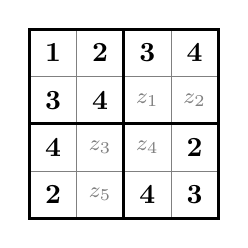
\begin{tikzpicture}[scale=0.6]
			\draw[gray] (0,0) grid (4,4);
			\draw[very thick] (0,0) rectangle (4,4);
			\draw[very thick] (2,0) -- (2,4);
			\draw[very thick] (0,2) -- (4,2);
			% Vorgaben, Zeile für Zeile von oben
			\foreach \c/\z in {0/1, 1/2, 2/3, 3/4} \node at (\c+0.5, 3.5) {\textbf{\z}};
			\foreach \c/\z in {0/3, 1/4} \node at (\c+0.5, 2.5) {\textbf{\z}};
			\foreach \c/\z in {0/4, 3/2} \node at (\c+0.5, 1.5) {\textbf{\z}};
			\foreach \c/\z in {0/2, 2/4, 3/3} \node at (\c+0.5, 0.5) {\textbf{\z}};
			% leere Zellen
			\node[gray] at (2.5, 2.5) {\footnotesize $z_1$};
			\node[gray] at (3.5, 2.5) {\footnotesize $z_2$};
			\node[gray] at (1.5, 1.5) {\footnotesize $z_3$};
			\node[gray] at (2.5, 1.5) {\footnotesize $z_4$};
			\node[gray] at (1.5, 0.5) {\footnotesize $z_5$};
		\end{tikzpicture}
	\end{minipage}%
	\hfill
	\begin{minipage}[c]{0.7\textwidth}
		\centering
		\begin{forest}
			for tree={
				draw, rounded corners=2pt, font=\footnotesize, inner sep=2pt,
				l sep=5mm, s sep=8mm, edge={->}
			}
			[Vorgaben, name=wurzel, label={[font=\tiny, text=gray]right:0}
				[{$z_1 = 1$}, name=sack1, fill=red!15, label={[font=\tiny, text=gray]right:1}]
				[{$z_1 = 2$}, label={[font=\tiny, text=gray]right:2}
					[{$z_2 = 1$}, name=knoten, label={[font=\tiny, text=gray]right:3}
						[{$z_3 = 1$}, name=sack2, fill=red!15, label={[font=\tiny, text=gray]right:4}]
						[{$z_3 = 3$}, label={[font=\tiny, text=gray]right:5}
							[{$z_4 = 1$}, label={[font=\tiny, text=gray]right:6}
								[{$z_5 = 1$}, fill=green!20, label={[font=\tiny, text=gray]right:7}]
							]
						]
					]
				]
			]
			\draw[->, dashed, red!70!black] (sack1.north west) to[bend left=30] (wurzel.west);
			\draw[->, dashed, red!70!black] (sack2.north west) to[bend left=30] (knoten.west);
		\end{forest}
	\end{minipage}
	\caption[Suchbaum des Backtrackings für ein $4 \times 4$-Sudoku]{Links ein $4 \times 4$-Sudoku mit Vorgaben (fett) und den leeren Zellen $z_1$ bis $z_5$, 
	rechts sein vollständiger Suchbaum. Rot markiert sind Sackgassen, grün die Lösung, 
	gestrichelt die Rücksprünge. Die grauen Zahlen geben die Reihenfolge an, 
	in der die Tiefensuche die Knoten besucht.}
	\label{fig:bt-suchbaum}
\end{figure}

% ----------------------------------------------------------------------------
\subsection{Algorithmus und Implementierung}\label{sec:bt-algorithmus}

Die Implementierung im Modul \texttt{naive.py} umfasst eine rekursive und eine iterative Variante 
desselben Verfahrens sowie einen Generator für die Visualisierung. 
Alle durchlaufen die Zellen zeilenweise, probieren die Ziffern aufsteigend von 1 bis 9 
und durchsuchen damit denselben Suchbaum in derselben Reihenfolge. 
Zur Abgrenzung von den Heuristiken in Abschnitt~\ref{sec:bt-heuristiken} 
wird diese Vorgehensweise als \emph{naives Backtracking} bezeichnet.

\begin{algorithm}[hbt]
	\caption{Rekursives Backtracking (\texttt{solve})}\label{alg:bt-rekursiv}
	\begin{algorithmic}[1]
		\Function{Solve}{$G, r, c$} \Comment{Gitter $G$, aktuelle Zelle $(r, c)$, Indizes 0 bis 8}
			\If{$r = 9$} \Return \textbf{true} \Comment{alle Zeilen belegt}
			\EndIf
			\If{$c = 9$} \Return \Call{Solve}{$G, r + 1, 0$} \Comment{weiter in der nächsten Zeile}
			\EndIf
			\If{$G[r][c] \neq 0$} \Return \Call{Solve}{$G, r, c + 1$} \Comment{Vorgabe überspringen}
			\EndIf
			\For{$z \gets 1, \dots, 9$}
				\If{\Call{Valid}{$G, r, c, z$}}
					\State $G[r][c] \gets z$
					\If{\Call{Solve}{$G, r, c + 1$}} \Return \textbf{true}
					\EndIf
					\State $G[r][c] \gets 0$ \Comment{Rücksprung}
				\EndIf
			\EndFor
			\State \Return \textbf{false}
		\EndFunction
	\end{algorithmic}
\end{algorithm}

Die rekursive Variante (Algorithmus~\ref{alg:bt-rekursiv}) erhält das Gitter und die aktuelle Zelle. 
Sie überspringt Vorgaben, wechselt am Zeilenende in die nächste Zeile und meldet Erfolg, 
sobald sie hinter der letzten Zeile angekommen ist. 
In einer leeren Zelle probiert sie nacheinander jede zulässige Ziffer und setzt die Suche rekursiv mit der nächsten Zelle fort. 
Scheitert dieser Aufruf, wird die Zelle wieder geleert (Zeile~9). 
Sind alle Ziffern erfolglos, gibt der Aufruf das Scheitern an seinen Aufrufer zurück, 
der daraufhin seine nächste Ziffer probiert. 
Die Zulässigkeitsprüfung \textsc{Valid} (\texttt{is\_valid\_number}) betrachtet nur Zeile, Spalte und Block der neuen Zelle: 
Da der bisherige Zustand konsistent ist, kann ein Widerspruch nur dort entstehen. 
Der Prüfaufwand pro Knoten ist damit konstant. 
Vor der Suche wird mit \texttt{is\_valid} einmalig geprüft, ob die Vorgaben widerspruchsfrei sind 
(siehe Abschnitt~\ref{sec:bt-korrektheit}).

Bei der Rekursion liegt der Zustand der Suche implizit auf dem Call-Stack, 
wobei jeder aktive Aufruf einem Knoten auf dem Pfad von der Wurzel zum aktuellen Zustand entspricht. 
Die iterative Variante \texttt{stack\_solve} macht diesen Stack explizit und ersetzt die Rekursion durch eine Schleife. 
Dazu werden die leeren Zellen $z_1, \dots, z_k$ vorab bestimmt. 
Ein Stackeintrag $(i, z)$ hält fest, dass die Zelle $z_i$ zuletzt die Ziffer $z$ erhalten hat. 
In jedem Durchlauf wird der oberste Eintrag entnommen und ab der Ziffer $z + 1$ nach der nächsten zulässigen Ziffer gesucht. 
Gelingt dies, kommt der aktualisierte Eintrag zurück auf den Stack und darüber ein neuer Eintrag für die Zelle $z_{i+1}$. 
Andernfalls bleibt der Eintrag entfernt, und der nächste Durchlauf setzt bei der vorherigen Zelle fort, 
was dem Rücksprung entspricht. 
Ist der Stack leer, sind alle Alternativen erschöpft und das Sudoku ist unlösbar.

Der eigen implementierte, explizite Stack hat die zwei folgenden Vorteile: 
Zum einen ist die Suche nicht durch die maximale Rekursionstiefe begrenzt, was bei $9 \times 9$-Sudokus zwar unkritisch ist, 
bei größeren Varianten aber relevant wird. 
Vor allem aber liegt der Suchzustand jederzeit vollständig vor, sodass die Suche nach jedem Schritt unterbrochen werden kann. 
Der Generator \texttt{solve\_steps} baut auf dieses Prinzip auf. 
Die Funktion gibt für jeden Schritt die jeweilige Aktion zurück mitsamt einer Kopie des Gitters. 

% ----------------------------------------------------------------------------
\subsection{Korrektheit, Vollständigkeit und Terminierung}\label{sec:bt-korrektheit}

Um die Lösbarkeit zu entscheiden, muss der Backtracker korrekt, vollständig und terminierend sein.

\emph{Korrektheit:} Da nur Ziffern gesetzt werden, die \textsc{Valid} erlaubt, 
und die Vorgaben vorab mit \texttt{is\_valid} geprüft werden, ist jeder erreichte Zustand konsistent. 
Meldet der Algorithmus Erfolg, sind alle $k$ Zellen belegt, es liegt also eine Lösung vor. 
Ohne die Vorabprüfung würde ein vollständig ausgefülltes, aber ungültiges Gitter als lösbar gemeldet.

\emph{Vollständigkeit:} Wegen der Monotonie aus Abschnitt~\ref{sec:bt-suchbaum} 
verwirft das Pruning nur Teilbäume ohne Lösung. Alle übrigen Knoten durchläuft die Tiefensuche systematisch. 
Eine existierende Lösung wird daher gefunden, 
und dass das Sudoku andernfalls unlösbar ist wird erst nach Durchsuchen des gesamten Baums gemeldet.

\emph{Terminierung:} Der Suchbaum ist endlich, da seine Tiefe höchstens $k$ und sein Verzweigungsgrad höchstens neun beträgt. 
Weil jede Zelle ihre Ziffern aufsteigend ab der zuletzt probierten durchläuft, wird kein Zustand doppelt erzeugt.

Der Backtracker hält somit auf jeder Eingabe mit der korrekten Antwort 
und ist ein Entscheidungsverfahren für die Sprache der lösbaren Sudokus aus Abschnitt~\ref{sec:csp}.

% ----------------------------------------------------------------------------
\subsection{Laufzeit- und Speicherkomplexität}\label{sec:bt-komplexitaet}

Da der Prüfaufwand pro Knoten konstant ist (Abschnitt~\ref{sec:bt-algorithmus}), 
bestimmt die Anzahl der besuchten Knoten die Laufzeit. 
Im ungünstigsten Fall wird der gesamte Suchbaum mit höchstens
\begin{equation}
	\sum_{i=0}^{k} 9^i = \frac{9^{k+1} - 1}{8} \in O(9^k)
\end{equation}
Knoten durchlaufen. Für das $9 \times 9$-Sudoku fester Größe ist diese Aussage 
nur eingeschränkt aussagekräftig (Abschnitt~\ref{sec:komplexitaet}). 
Beim verallgemeinerten $n^2 \times n^2$-Sudoku beträgt der Verzweigungsgrad bis zu $n^2$, 
die Laufzeit liegt also in $O(n^{2k})$ und wächst exponentiell mit der Anzahl der leeren Zellen. 
Wie viele Knoten tatsächlich besucht werden, hängt von der Instanz und der Suchreihenfolge ab 
und wird in Kapitel~\ref{sec:evaluation} empirisch untersucht.

Der Speicherbedarf ist dagegen gering: Neben dem Gitter wird nur der Pfad von der Wurzel zum aktuellen Knoten 
mit höchstens $k$ Stackeinträgen gespeichert, also $O(k)$. 
Eine Breitensuche müsste dagegen ganze Ebenen mit bis zu $9^i$ Zuständen vorhalten.

Dem exponentiellen Suchaufwand steht die Überprüfung einer Lösung gegenüber, 
die \texttt{is\_solved} in polynomieller Zeit leistet. 
Diese Asymmetrie entspricht der Einordnung in NP aus Abschnitt~\ref{sec:komplexitaet}: 
Das Backtracking ersetzt das nichtdeterministische Raten einer Lösung durch systematisches Ausprobieren 
und bezahlt dies mit exponentiellem Aufwand. 
Da das verallgemeinerte Sudoku NP-vollständig ist \vgl{yato2003}, 
existiert unter der Annahme $\mathrm{P} \neq \mathrm{NP}$ kein Algorithmus mit polynomieller Laufzeit. 
Der exponentielle Worst Case ist somit eine Eigenschaft des Problems und nicht des Verfahrens. 
Verbessern lässt sich jedoch der Aufwand typischer Instanzen durch eine geschicktere Suchreihenfolge, 
wie der folgende Abschnitt zeigt.

% ----------------------------------------------------------------------------
\subsection{Heuristiken zur Verkleinerung des Suchbaums}\label{sec:bt-heuristiken}

Am exponentiellen Worst Case lässt sich nach Abschnitt~\ref{sec:bt-komplexitaet} nichts ändern. 
Der Aufwand für eine konkrete Instanz hängt jedoch stark davon ab, in welcher Reihenfolge die Zellen belegt werden. 
Das naive Backtracking belegt sie in einer festen, zeilenweisen Reihenfolge, unabhängig vom aktuellen Zustand. 
Im Modul \texttt{heuristic.py} sind zwei Heuristiken aus dem Bereich der Constraint-Satisfaction-Probleme umgesetzt, 
die die Suche an den aktuellen Zustand anpassen \vgl{russell2021}. 
Beide lassen sich unabhängig voneinander zuschalten.

\emph{\ac{MRV}:} Statt der nächsten Zelle in fester Reihenfolge wird die leere Zelle 
mit den wenigsten zulässigen Ziffern, den sogenannten Kandidaten, als Nächstes belegt. 
Dahinter steht das Fail-First-Prinzip \vgl{haralick1980}: 
Muss ein Zweig scheitern, soll er möglichst früh und damit möglichst nah an der Wurzel scheitern, 
da so der größte Teilbaum eingespart wird. 
Hat eine Zelle nur einen Kandidaten, ist ihre Belegung erzwungen und der Baum verzweigt sich an dieser Stelle nicht. 
Hat eine Zelle keinen Kandidaten, wird die Sackgasse sofort erkannt, statt zuvor noch weitere Zellen zu belegen. 
Der Suchbaum ist weiterhin wie in Abschnitt~\ref{sec:bt-suchbaum} definiert, 
nur wird die nächste Zelle $z_{i+1}$ nun abhängig vom aktuellen Zustand gewählt. 
Korrektheit, Vollständigkeit und Terminierung aus Abschnitt~\ref{sec:bt-korrektheit} bleiben daher erhalten.

\emph{\ac{FC}:} Nach jeder gesetzten Ziffer wird geprüft, 
ob in der Zeile, der Spalte oder dem Block der Zelle eine leere Zelle ohne Kandidaten entstanden ist. 
In diesem Fall wird die Ziffer sofort zurückgenommen, 
auch wenn die betroffene Zelle in der festen Reihenfolge erst viel später an der Reihe wäre.

\begin{table}[hbt]
	\centering
	\caption[Gesetzte Ziffern bis zur ersten Lösung: naives Backtracking und Heuristiken]{Gesetzte Ziffern bis zur ersten Lösung für das naive Backtracking und die Heuristiken.
	Die Suche wurde nach $500\,000$ gesetzten Ziffern abgebrochen.} {\emph{Eigene Messung}}
	\label{tab:bt-heuristiken}
	\begin{tabular}{lrrrrr}
		\toprule
		Sudoku & leere Zellen & naiv & naiv + \acs{FC} & \acs{MRV} & \acs{MRV} + \acs{FC} \\
		\midrule
		Wikipedia                      & 51 & $4\,208$     & $516$        & $51$       & $51$ \\
		AI Escargot                    & 58 & $8\,969$     & $5\,421$     & $217$      & $217$ \\
		Inkala 2012                    & 60 & $49\,558$    & $22\,067$    & $10\,101$  & $10\,101$ \\
		Norvig \glqq hard1\grqq{}      & 64 & $>500\,000$  & $>500\,000$  & $481$      & $481$ \\
		Anti-Backtracking              & 64 & $>500\,000$  & $>500\,000$  & $45\,267$  & $45\,267$ \\
		Leicht für Backtracking	       & 57 & $992$        & $336$        & $3\,220$   & $3\,220$ \\
		Unlösbares Sudoku              & 72 & $>500\,000$  & $>500\,000$  & $0$        & $0$ \\
		\bottomrule
	\end{tabular}
\end{table}

Tabelle~\ref{tab:bt-heuristiken} vergleicht die Anzahl gesetzter Ziffern, also der besuchten Knoten, 
für einige Sudokus aus der Sammlung des Projekts. 
Die Werte lassen sich mit dem Skript \texttt{report.py} reproduzieren. 
Beim Wikipedia-Sudoku setzt \ac{MRV} genau 51 Ziffern für 51 leere Zellen: 
Jede Belegung ist erzwungen, und der Suchbaum besitzt keine einzige Verzweigung. 
Beim Sudoku \glqq hard1\grqq{} sinkt der Aufwand von rund 9,7 Millionen gesetzten Ziffern 
ohne Abbruch auf 481, beim Anti-Backtracking-Sudoku von rund 69 Millionen auf etwa $45\,000$. 
Am deutlichsten zeigt sich das Fail-First-Prinzip beim unlösbaren Sudoku. 
Seine letzte Zelle besitzt von Beginn an keinen Kandidaten. 
\ac{MRV} erkennt das, ohne eine einzige Ziffer zu setzen, 
während das naive Verfahren diese Zelle erst erreicht, wenn alle 71 davorliegenden Zellen belegt sind, und dies für jede mögliche Belegung erneut.

Zwei Beobachtungen fallen auf. 
Erstens setzt \ac{MRV} mit \ac{FC} in allen Fällen genau so viele Ziffern wie \ac{MRV} allein. 
Eine Zelle ohne Kandidaten, die \ac{FC} erkennen würde, ist genau die Zelle, die \ac{MRV} als Nächstes wählt 
und an der die Suche ohne weitere Platzierung scheitert. 
\ac{FC} lohnt sich daher nur bei einer festen Reihenfolge. 
Zweitens ist eine Heuristik keine Garantie: Beim Sudoku \glqq Leicht für Backtracking\grqq{} 
benötigt \ac{MRV} mit $3\,220$ gesetzten Ziffern mehr als das Dreifache des naiven Verfahrens. 
\ac{MRV} entscheidet nur nach einem lokalen Kriterium und kann dadurch in größere Teilbäume geraten, 
die die feste Reihenfolge zufällig umgeht. 
Zudem ist ein Knoten bei \ac{MRV} teurer, da die Kandidaten aller leeren Zellen bestimmt werden müssen. 
Wie sich das auf die Laufzeit auswirkt, wird in Kapitel~\ref{sec:evaluation} untersucht.

% TODO: ref auf das Laufzeit Kapitel wenn es soweit ist
Aus Sicht der theoretischen Informatik ändern die Heuristiken nur die Reihenfolge der Suche, nicht den Suchraum. 
Die obere Schranke $O(9^k)$ aus Abschnitt~\ref{sec:bt-komplexitaet} bleibt bestehen, 
und unter der Annahme $\mathrm{P} \neq \mathrm{NP}$ kann keine Heuristik die Laufzeit allgemein polynomiell machen. 
Heuristiken verkleinern den Suchbaum typischer Instanzen um Größenordnungen, die Komplexitätsklasse des Problems ändern sie nicht.

% ----------------------------------------------------------------------------
\subsection{Abschätzung der Suchbaumgröße nach Knuth}\label{sec:bt-knuth}

Tabelle~\ref{tab:bt-heuristiken} zeigt, dass sich der Aufwand selbst bei ähnlich vielen leeren Zellen 
um mehrere Größenordnungen unterscheiden kann. 
Ob eine Suche nach Millisekunden oder erst nach Jahren endet, ist vorab meist nicht erkennbar. 
\textcite{knuth1975} schlug dafür ein Monte-Carlo-Verfahren vor, das die Größe eines Backtracking-Suchbaums schätzt, 
ohne ihn zu durchlaufen. Es ist im Modul \texttt{estimation.py} umgesetzt.

Das Verfahren folgt einem zufälligen Pfad von der Wurzel bis zu einem Blatt 
und wählt in jedem Knoten eines der Kinder gleichverteilt aus. 
Bezeichnet $d_j$ die Anzahl der Kinder des $j$-ten Knotens auf diesem Pfad, 
beginnend mit der Wurzel, so ist die Schätzung für einen Pfad mit $t$ inneren Knoten
\begin{equation}
	X = 1 + d_1 + d_1 d_2 + \dots + d_1 d_2 \cdots d_t.
\end{equation}
Die Intuition dahinter ist, dass alle Geschwister eines besuchten Knotens als gleich groß angenommen werden. 
Hat die Wurzel zwei Kinder, werden auf der ersten Ebene zwei Knoten geschätzt. 
Hat das gewählte Kind wieder zwei Kinder, werden auf der zweiten Ebene $2 \cdot 2 = 4$ Knoten geschätzt. 
Als Gesamtschätzung dient der Mittelwert über viele unabhängige Pfade.

Diese Schätzung ist erwartungstreu. 
Ein Knoten $v$ in Tiefe $j$ liegt mit der Wahrscheinlichkeit $p_v = 1/(d_1 \cdots d_j)$ auf dem zufälligen Pfad 
und trägt in diesem Fall genau den Summanden $d_1 \cdots d_j = 1/p_v$ zu $X$ bei. 
Für den Erwartungswert über alle Knoten $v$ des Suchbaums $T$ folgt daher
\begin{equation}
	E[X] = \sum_{v \in T} p_v \cdot \frac{1}{p_v} = |T|.
\end{equation}
Für den Suchbaum aus Abbildung~\ref{fig:bt-suchbaum} gibt es folgende drei mögliche Pfade. 
Der Pfad über $z_1 = 1$ wird mit Wahrscheinlichkeit $\frac{1}{2}$ gewählt und liefert $X = 1 + 2 = 3$, 
die beiden Pfade über $z_3 = 1$ und $z_3 = 3$ mit Wahrscheinlichkeit je $\frac{1}{4}$ 
liefern $X = 9$ und $X = 17$. 
Der Erwartungswert $\frac{1}{2} \cdot 3 + \frac{1}{4} \cdot 9 + \frac{1}{4} \cdot 17 = 8$ 
entspricht genau den acht Knoten des Baums.

\begin{table}[hbt]
	\centering
	\caption[Exakte Suchbaumgröße und Schätzung nach Knuth]{Exakte Größe des vollständigen Suchbaums und Schätzung nach Knuth aus $1000$ Pfaden.
	Die exakte Zählung wurde nach $500\,000$ Knoten abgebrochen.} {\emph{Eigene Messung}}
	\label{tab:bt-knuth}
	\small
	\setlength{\tabcolsep}{4pt}
	\begin{tabular}{llrrrrr}
		\toprule
		Sudoku & Reihenfolge & exakt & Schätzung & Std.-Fehler & min. $X$ & max. $X$ \\
		\midrule
		Wikipedia         & naiv     & $4\,632$     & $5\,546$      & $1\,187$      & $64$      & $722\,350$ \\
		                  & \acs{MRV} & $52$        & $52$          & $0$           & $52$      & $52$ \\
		AI Escargot       & naiv     & $18\,885$    & $40\,462$     & $25\,714$     & $65$      & $2{,}5 \cdot 10^{7}$ \\
		                  & \acs{MRV} & $2\,232$    & $2\,088$      & $150$         & $33$      & $55\,433$ \\
		Anti-Backtracking & naiv     & $>500\,000$  & $5{,}2 \cdot 10^{7}$ & $2{,}3 \cdot 10^{7}$ & $8\,282$ & $1{,}6 \cdot 10^{10}$ \\
		                  & \acs{MRV} & $73\,483$   & $64\,495$     & $9\,013$      & $46$      & $4{,}3 \cdot 10^{6}$ \\
		\bottomrule
	\end{tabular}
\end{table}

Tabelle~\ref{tab:bt-knuth} vergleicht die Schätzung mit der exakten Größe des vollständigen Suchbaums, 
die durch Zählen aller Knoten mit \texttt{tree\_size} bestimmt wurde. 
Anders als in Tabelle~\ref{tab:bt-heuristiken} umfasst der vollständige Baum auch alle Knoten nach der ersten Lösung. 
Er entspricht damit dem Aufwand einer erschöpfenden Suche, wie sie bei unlösbaren Sudokus nötig ist, aber auch beim Zählen aller Lösungen oder beim Prüfen, ob eine Lösung eindeutig ist. 
Für die Bäume mit \ac{MRV} liegt die Schätzung nahe am exakten Wert. 
Beim Wikipedia-Sudoku verzweigt der Baum nie, sodass jeder Pfad den exakten Wert liefert.

In unbalancierten Bäumen, wie sie das naive Verfahren erzeugt, schwanken die einzelnen Schätzungen dagegen stark. 
Die meisten Pfade enden schnell in einer Sackgasse, 
während seltene Pfade in einen riesigen Teilbaum führen und dann extrem große Werte liefern. 
Die Verteilung von $X$ ist dadurch stark rechtsschief, 
und der Standardfehler des Mittelwerts sinkt nur mit $1/\sqrt{N}$ in der Anzahl $N$ der Pfade. 
Beim Sudoku AI Escargot überschätzt der Mittelwert die exakte Größe um mehr als das Doppelte, 
weil ein einzelner Pfad allein rund 25 Millionen Knoten schätzt. 
Beim Anti-Backtracking-Sudoku reichen die Einzelschätzungen über sechs Größenordnungen. 
Der Mittelwert von rund 52 Millionen liegt sogar unter den 69 Millionen Knoten, 
die das naive Verfahren bereits bis zur ersten Lösung besucht. 
Er unterschätzt also deutlich, weil die seltenen, sehr großen Werte bei $1000$ Pfaden kaum gezogen werden.

Damit zeigt sich die zentrale Schwäche des Verfahrens: 
Gerade bei sehr großen Bäumen, für die eine Vorhersage am wertvollsten wäre, ist die Schätzung am unzuverlässigsten. 
Für eine Einordnung der Größenordnung genügt sie dennoch. 
Für das unlösbare Sudoku schätzt das Verfahren in naiver Reihenfolge rund $8 \cdot 10^{16}$ Knoten 
und sagt damit richtig voraus, dass die naive Suche praktisch nicht endet, 
während der Baum mit \ac{MRV} aus nur einem Knoten besteht.

% ----------------------------------------------------------------------------
